\begin{refsection}

\chapter{Resumo Estendido em Língua Portuguesa}\label{appendix:pt_estendido}
\setlength{\absparsep}{18pt} % ajusta o espaçamento dos parágrafos do resumo
{\normalsize\noindent{\textbf{Título}: Título do trabalho em língua portuguesa}\\}
{\normalsize{\textbf{Autor:} Nome Completo do Autor}\\}
{\normalsize{\textbf{Orientador:} Nome Completo do Orientador}\\}
%{\setfonttimes\normalsize{\textbf{Coorientador:} Nome Completo do Coorientador}\\}
{\normalsize{\textbf{Programa de Pós-Graduação em Sistemas Mecatrônicos}}\\}
{\normalsize{\textbf{Brasília, 14 de setembro de 2022}}\\\\}
{\normalsize\noindent{\textbf{Palavras-chave:} Palavra chave 1. Palavra chave 2. Palavra chave 3. Palavra chave 4.}}

\vspace{-5mm}

\vspace{14pt}

\section*{Introdução}
Para dissertações ou teses em inglês, é necessário que o resumo em português seja no formato estendido. Trata-se de um formato com divisão própria de seções, como aqui exemplificado. A primeira seção deve ser denominada \emph{Introdução}.

O resumo estendido deve contar com uma lista própria de referências, citadas ao longo do resumo, como neste exemplo \cite{talbot2012}. Procure selecionar as referências mais importantes da sua lista principal. Pode usar a mesma 'chave' ou nome da referencia bibliografica usada no corpo do documento \cite{ibge1993}. É possível colocar as referências do resumo estendido em um arquivo bib diferente, mas não é necessário (no presente exemplo, as referências estão todas num só arquivo bib).

\section*{Materiais e Métodos}
O resumo estendido deve ter entre 4 e 6 páginas, pode incluir figuras e tabelas próprias, como no exemplo da Figura~\ref{fig:appendix_grafico}, mas lembre-se de usar "[]" após o "caption" e antes do "{}" para evitar que esta figura vá para a lista de figuras.

\begin{figure}[htb]
	\begin{center}
	    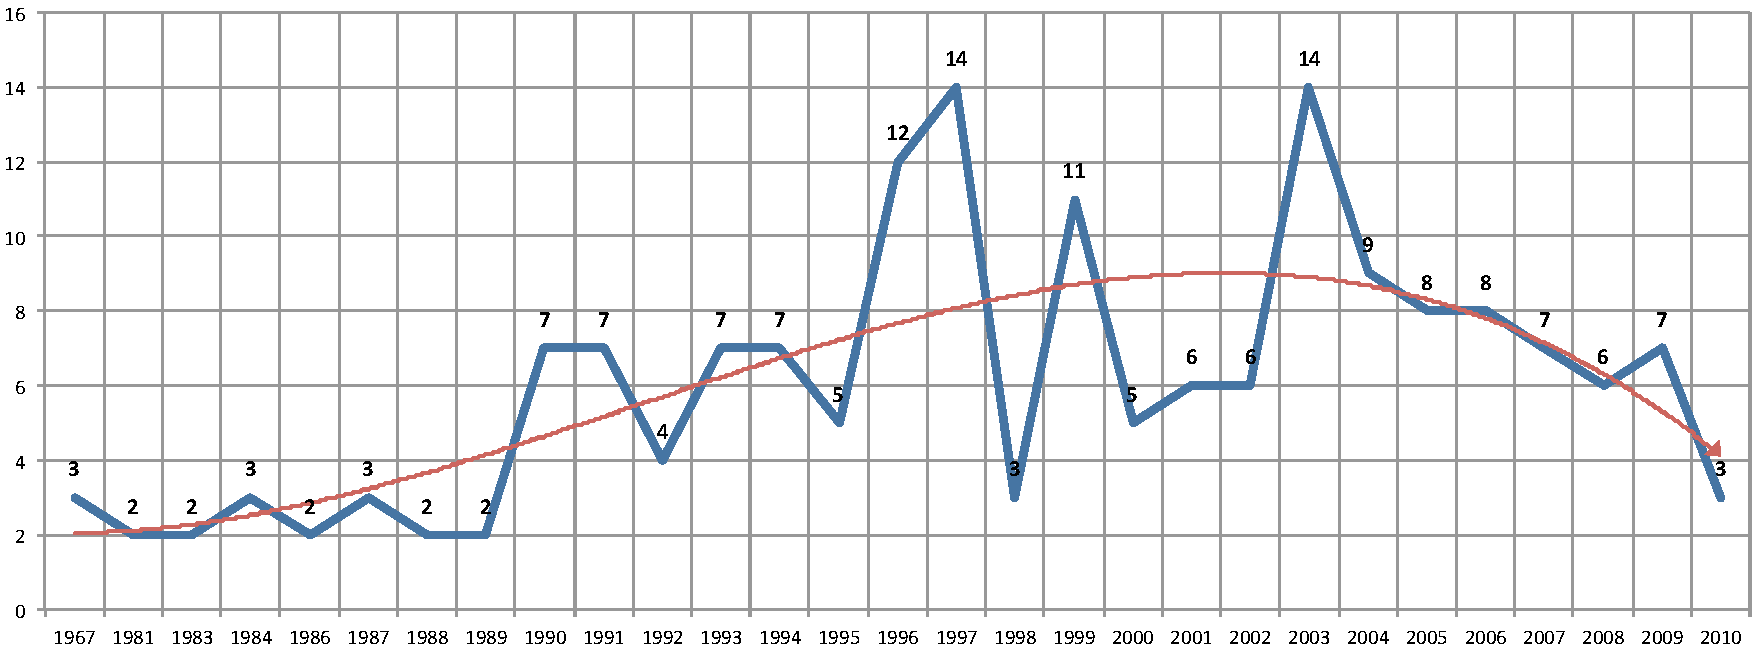
\includegraphics[scale=0.5]{img-grafico.pdf}
	\end{center}
	\caption[]{Este grafico novamente.}
    \label{fig:appendix_grafico}
	\legend{Fonte: \textcite[24]{araujo2012}}
\end{figure}

\section*{Resultados e Discussões}
Escreva aqui os resultados mais importantes. 

Os resultados da simulação numérica mostraram que ...

\section*{Conclusão}
A última seção deve ser denominada \emph{Conclusão}. 

Escreva aqui as conclusões.

% ---
% Referências bibliográficas do resumo estendido
% ---

{\let\clearpage\relax
\defbibheading{bibresumoestendido}[\bibname]{\section*{#1}}
\cleardoublepage
\phantomsection
\tocprintchapternonum
\addcontentsline{}{section}{\texorpdfstring{\MakeTextUppercase{\bibname}}{\bibname}}
\printbibliography[heading=bibresumoestendido, title={Referências}]
\markboth{}{}
}

\end{refsection}

